% Chapter 1

\chapter{Resultados} % Main chapter title
\label{Cap_Res} % For referencing the chapter elsewhere, use \ref{Chapter1} 



\section{Datos recolectados}

%SDatos duros antes del análisis.
Antes de realizar los análisis esadísticos correspondientes para determinar si se encontró -o no- evidencia sólida del Efecto Espejo en nuestros experimentos, se exploró de manera exhaustiva los datos recopilados de la ejecución de los participantes, graficando su relación con diferentes variables inmersas en los mismoa.\\ 

%Se destaca la implrtancia de revisar los datos antes de someterlos a analisis estadísticos
Graficar los datos antes de someterlos a un análisis estadístico para elaborar conclusiones constituye una práctica recomendable en tanto que 1) se evalúa la pertinencia de los experimentos diseñados a la luz de las respuestas obtenidas por los participantes y 2) constituye un primer filtro para descartar la posibilidad de que los participantes estuvieren respondiendo de manera incongruente e inconsistente con las tareas presentadas, permitiéndonos tener una mayor confianza en las conclusiones que puedan extraerse de su análisis.\\

%Presentación de los controles graficados: Atención, El efecto del paso del tiempo y las variables externas en los estímulos. 
En este capítulo se presentan las gráficas correspondientes a la exploración de tres grandes tipos de correlaciones posibles que, de existir, podrían sugerir que los participantes no estuvieron respondiendo a la tarea de manera congruente con el diseño e interés de los experimentos, sino por influencia de factores externos a los mismos: 

\begin{itemize}
\item Emisión de trenes de respuesta.\\

El participante parece quedarse fijo en una sola respuesta a lo largo de varios ensayos, sugiriendo una dependencia entre la respuesta dada a cada ensayo y las respuestas emitidas en los ensayos inmediatamente anteriores.

\item Aprendizaje o Fatiga\\

La ejecución de los participantes cambia con  el paso del tiempo.

\item Sesgos o Preferencias.\\

Las propiedades de los estímulos diseñados influyen en las respuestas dadas por el participante o en su desempeño.  
\end{itemize}

Idealmente, en nuestros experimentos se esperaba que el desempeño de los participantes no mostrara cambios en función a ninguna característica de los estímulos construidos que no sea el número de círculos externos en las figuras de Ebbinghaus (la variable manipulada para la construcción de las condiciones de dificultad).






\subsection{Control 1: ¿Los participantes estaban poniendo atención a la tarea para emitir una respuesta?}

%Evaluando la atención: Que
Los experimentos realizados estuvieron compuestos de 640 ensayos a lo largo de los cuales los participantes tuvieron que 1) decidir si los estímulos presentados cumplían con la condición que se les solicitó detectar y 2) valorar su certidumbre sobre esta primer respuesta y asignarle un puntaje. Dada la extensión y lo demandante del procedimiento, la primer preocupación era que los participantes se agotaran y dejaran de poner atención a la tarea al emitir sus respuestas. Para controlar esta posibilidad, se revisaron las respuestas emitidas ensayo a ensayo para verificar que todas las opciones de respuesta fueran utilizadas para cada tarea planteada y que no se presentaran trenes de respuesta que pudieran sugerir una emisión de respuestas independiente del contenido de la tarea.\\

\begin{itemize}
\item Emisión de respuestas 'Sí/No' a lo largo del experimento.

Primero se graficaron las respuestas emitidas ensayo a ensayo durante la tarea de detección binaria ('Sí, los círculos son iguales', 'No, los círculos son diferentes'). El objetivo principal de estas gráficas fue el de detectar trenes de respuesta prolongados que, dada la aleatoriedad con que los estímulos fueron presentados por el programa, pudieran delatar un sesgo del participante a presionar una tecla en particular independientemente del estímulo a evaluar en pantalla.\\

%Participante representativo: Respuestas 'No' por 80 ensayos
La Figura~\ref{fig:Resp_E1_P1} ilustra la importancia de revisar los datos antes de incluirlos en el análisis estadístico y extraer conclusiones, al presentar las respuestas emitidas a la tarea de detección binaria por el Participante 1 del Experimento 2, quien pasó los primeros 80 ensayos del experimento respondiendo repetidamente a la tecla 'No'. Este tren de respuesta es lo suficientemente largo como para cuestionar la atención con que el Participante 1 estuvo respondiendo a la tarea.\\ 

\begin{figure}[th]
\centering
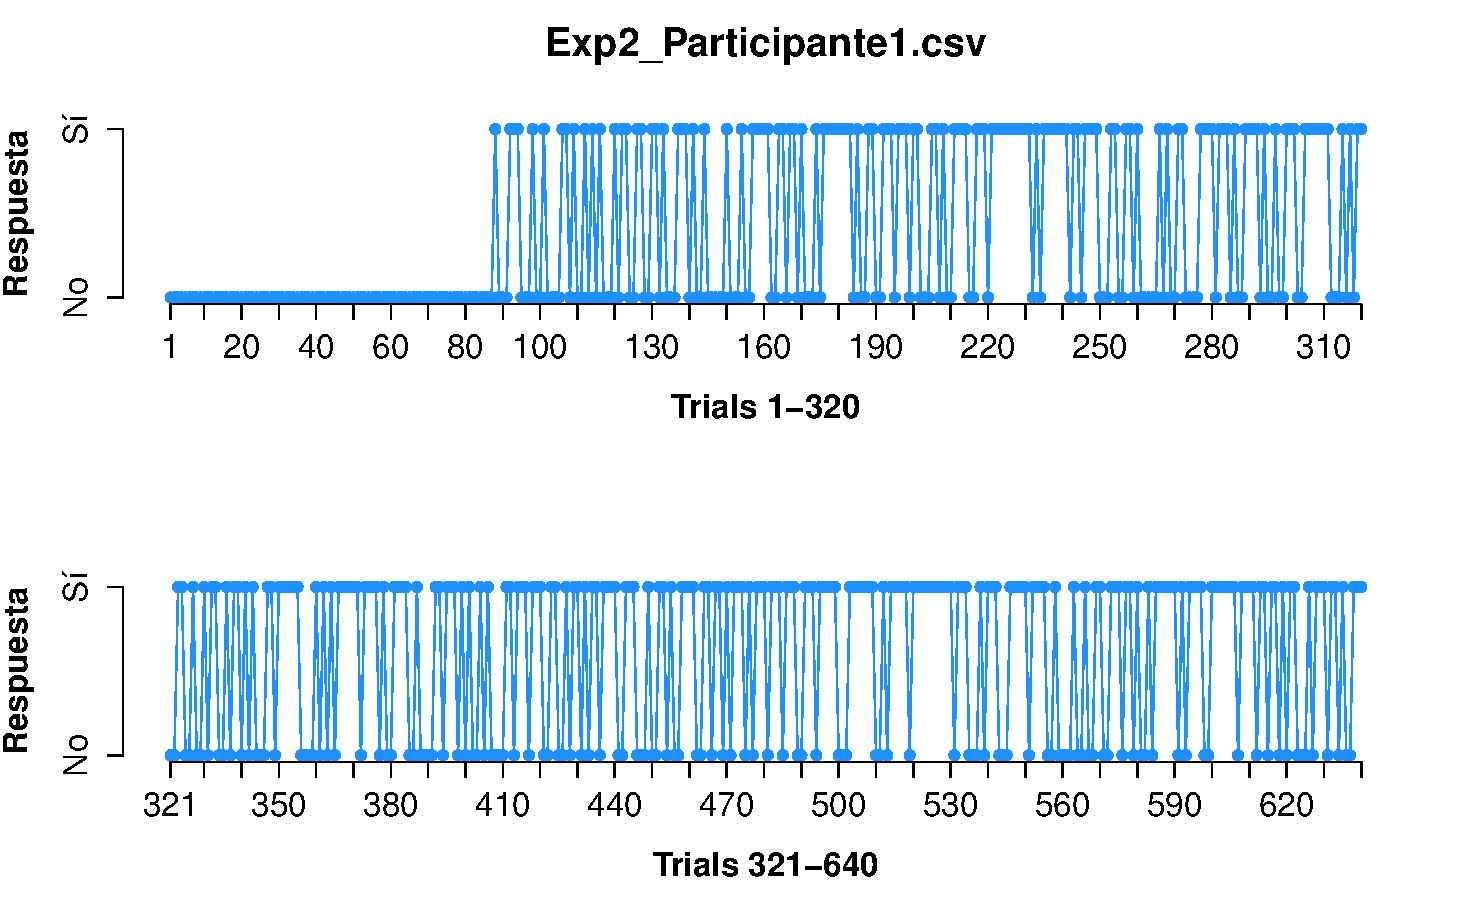
\includegraphics[width=0.60\textwidth]{Figures/Response_Exp2_P1} 
%\decoRule
\caption[Respuesta emitida por ensayo; ejemplo de participante sesgado]{Se muestran las respuestas ('Sí/No') emitidas en cada uno de los 640 ensayos del Experimento 1 por el Participante 1. La gráfica superior muestra los primeros 320 ensayos y la gráfica inferior, los 320 restantes. En el panel superior se aprecia con claridad un tren de respuesta que se extiende a lo largo de 80 ensayos, durante los cuales el Participante 1 sólo utilizó una de las opciones de respuesta.}
\label{fig:Resp_E1_P1}
\end{figure}

%Las gráficas correspondientes al resto de los participantes en los Experimentos 1 y 2, se muestran en las Figuras~\ref{fig:Response_P1} y \ref{fig:Response_E2}, respectivamente.\\

\item Correlación entre las respuestas 'Sí/No' emitidas y el tipo de estímulo presentado en cada ensayo.

A continuación, se graficaron las respuestas emitidas por los participantes en cada ensayo añadiendo indicadores que señalaran las características de los estímulos presentados; en concreto, si se trataba de una señal o ruido y si se trataba de un estímulo fácil o difícil.\\ 

Retomando el caso del Participante 1 del Experimento 2 presentado en la Figura~\ref{fig:Resp_E1_P1}, la Figura~\ref{fig:BiasResp_E1_P1} explora la posible correlación entre las respuestas registradas y el tipo de estímulo presentado en cada ensayo. Sin embargo, parece ser que el tren de 80 respuestas 'No' consecutivas se mantiene con independencia del tipo de estímulo presentado. Con base en dicha evidencia, se decidió eliminar al Participante 1 del Experimento 2 del análisis estadístico, pues se cree que se tiene razones suficientes para dudar de la atención que el participante estaba prestando al responder a la tarea.\\

\begin{figure}[th]
\centering
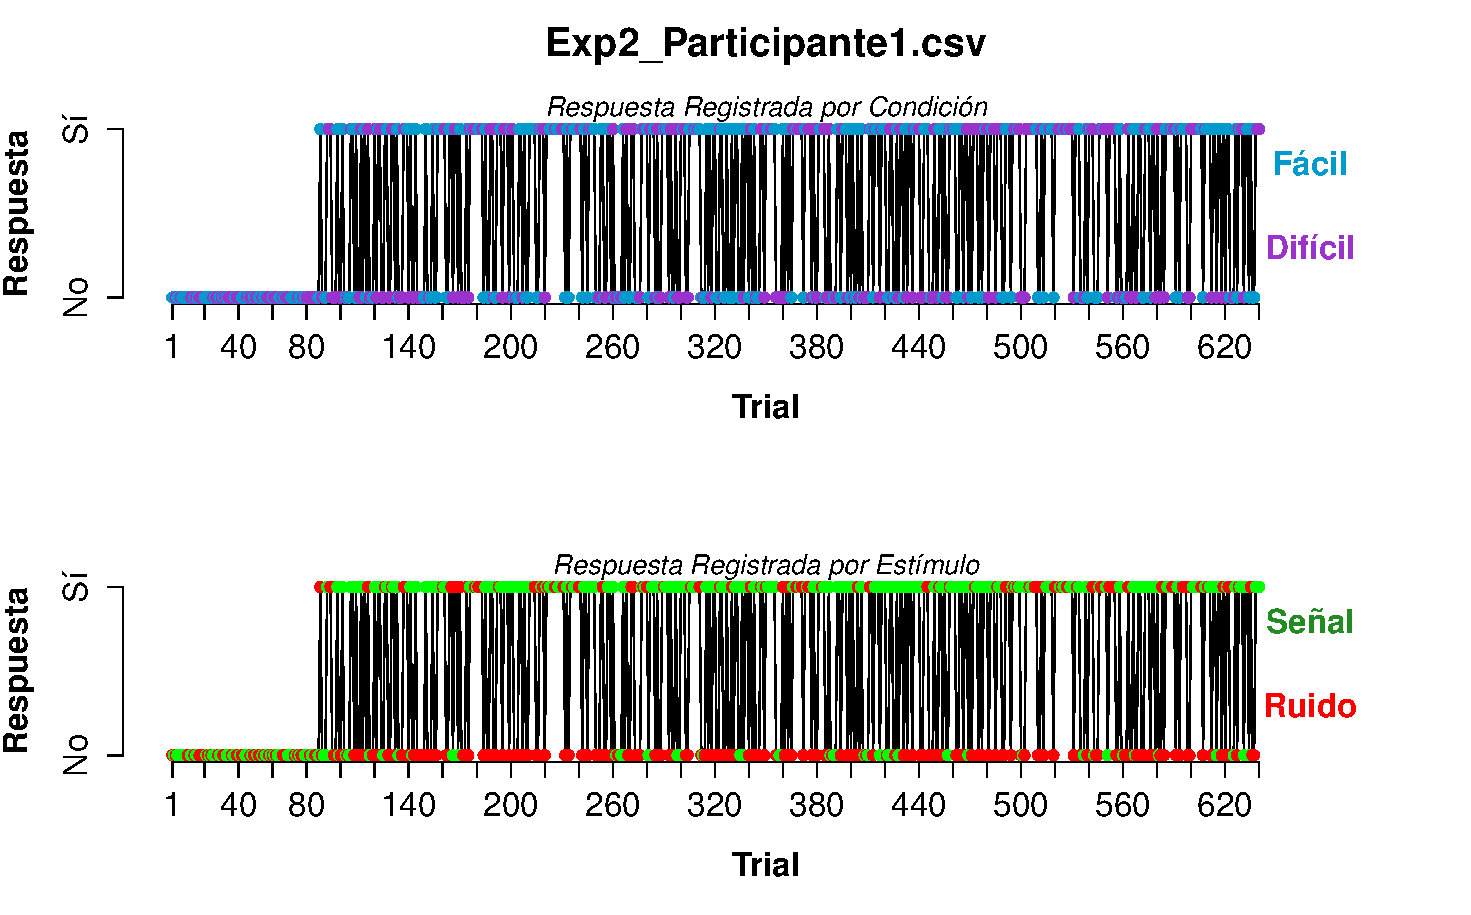
\includegraphics[width=0.60\textwidth]{Figures/BiasResp_Exp2_P1} 
%\decoRule
\caption[Respuesta por Tipo de Estimulo; ejemplo de participante sesgado]{Se muestran las respuestas registradas por el Participante 1 en cada uno de los ensayos del Experimento 2, indicando con diferentes colores el tipo de estímulo que se le mostraba en cada ocasión. En el panel superior se señala con colores violeta y azul si el estímulo presentado pertenecía a la categoría Difícil o Fácil, respectivamente. En el panel inferior se indica si se trataba de una señal o ruido, señalándolos con los colores verde y rojo, respectivamente.}
\label{fig:BiasResp_E1_P1}
\end{figure}

%Las Figuras~\ref{fig:BiasResp_E1} y () muestran las gráficas correspondientes al resto de los participantes en el Experimento 1 y 2, respectivamente.\\

\item Asignación de puntajes de confianza, ('1','2' y '3').

En la segunda fase de la tarea, los participantes tenían tres opciones de respuesta (teclas '1', '2' y '3') para señalar qué tanta confianza tenían sobre la respuesta previa ('poco seguro', 'más o menos seguro' o 'muy seguro', respectivamente). Las respuestas emitidas eran registradas por el programa de acuerdo a una escala mayor, (con valores del 1 al 6), que diferencía entre la confianza de haber rechazado correctamente un estímulo con ruido (e.g. '1, estoy seguro de que los círculos eran diferentes') y la confianza de haber identificado correctamente un estímulo con la señal a detectar (e.g '6, estoy seguro de que los círculos son iguales'), dejando los valores intermedios de la escala (3 y 4) para los puntajes que correlacionaran con una confianza baja en la respuesta emitida (e.g. '3, poco seguro de que los círculos eran diferentes' y '4, poco seguro de que los círculos eran iguales').\\

Tal y como se hizo para la tarea de detección binaria, se graficaron los puntajes de confianza asignados por los participantes en cada uno de los 640 ensayos que conformaron los experimentos. La Figura~\ref{fig:Rating_E2_P4} muestra los puntajes emitidos por el Participante 15 del Experimento 2 a lo largo de la tarea. Este participante, de acuerdo con lo que se esperaría de alguien que estuviere prestando atención a la tarea, utiliza todas las opciones de respuesta (teclas '1', '2' y '3'), siendo estas registradas por el programa de acuerdo con la respuesta dada a la tarea de detección binaria ('1' como '3' o '4', '2' como '2' o '5', '3' como '1' o '6'; dependiendo si la respuesta previa fue un 'no' o un 'sí', respectivamente).\\ 
 
\begin{figure}[th]
\centering
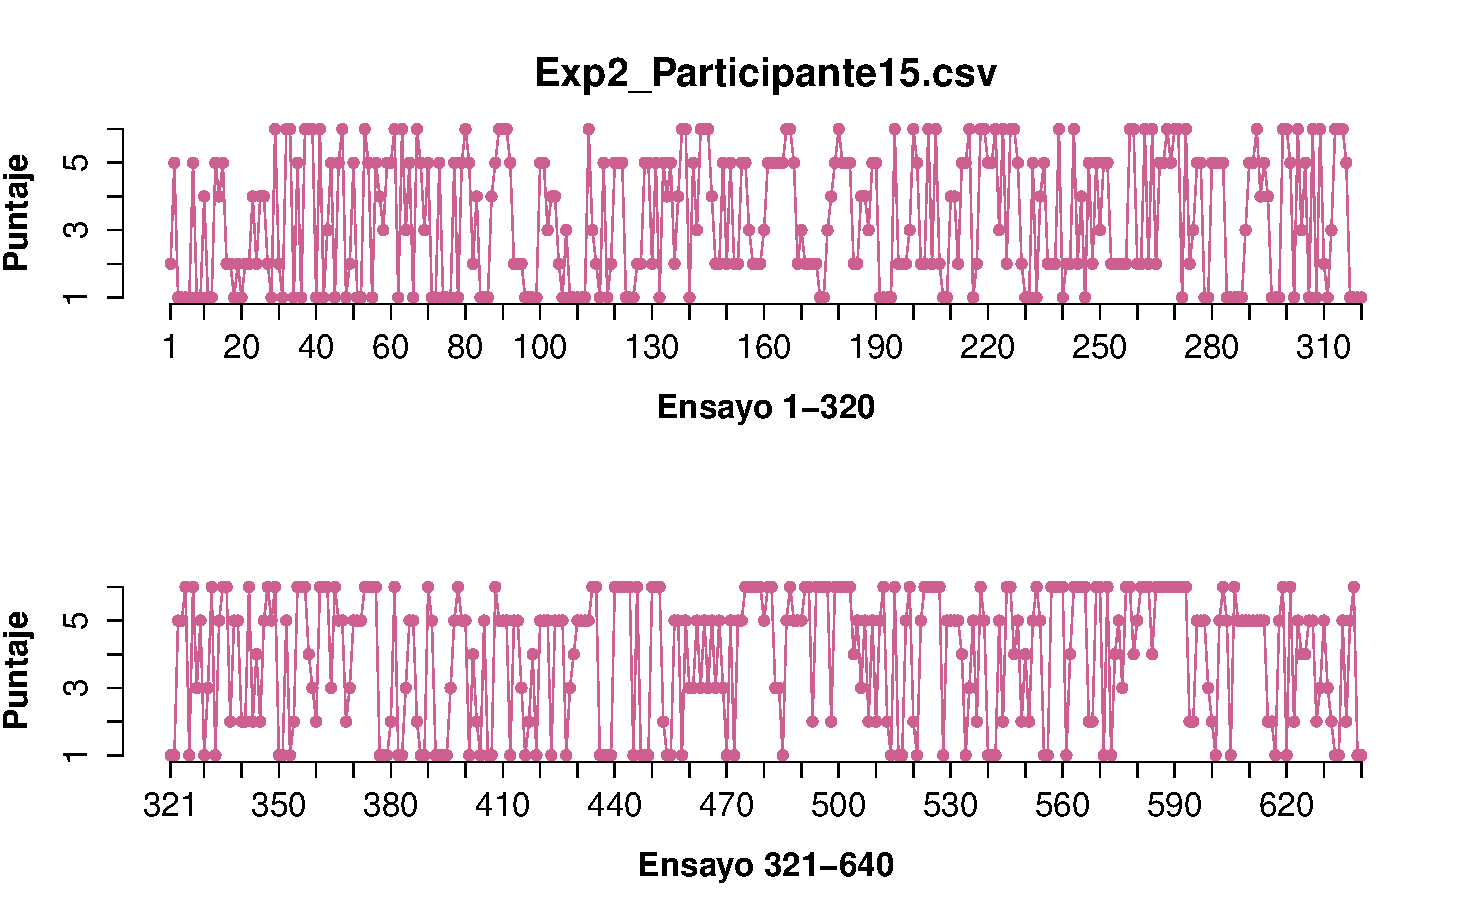
\includegraphics[width=0.60\textwidth]{Figures/Rating_Exp2_P15} 
%\decoRule
\caption[Asignacion Puntaje de confianza: Ejemplo]{Se muestran los puntajes de confianza asignados por el Participante 15 del Experimento 1 a las respuestas emitidas en la tarea binaria, durante cada uno de los 640 ensayos que conforman el experimento. El panel superior muestra los puntajes asignados en los primeros 320 ensayos del experimento; el panel inferior, muestra los 320 restantes.}
\label{fig:Rating_E2_P4}
\end{figure}

%El registro ensayo a ensayo de los puntajes de confianza asignados por el resto de los participantes en los Experimentos 1 y 2 se muestran en las Figuras~\ref{fig:Rating_E1} y \ref{fig:Rating_E2}, respectivamente.\\

\end{itemize}




\subsection{Control 2: ¿La duración del experimento tuvo un impacto en la ejecución de los participantes?}

La fatiga y la habituación a la ilusión constituyen dos grandes preocupaciones que se tuvieron a la hora de diseñar los experimentos, mismas que se buscó prevenir añadiendo controles tales como la pantalla de espera entre ensayos (para dar a los participantes la oportunidad de estirarse o descansar, hasta que se sintieran listos para atender al siguiente estímulo) y la exposición limitada a los estímulos a comparar por 1.5 segundos (para preveer que la ilusión perdiera fuerza mientras más tiempo pasaran los participantes estudiando la figura). Teniendo esto en mente, se realizó un segundo conjunto de gráficas para verificar que efectivamente el desempeño de los participantes no mostraran indicios de un posible efecto de la fatiga  o de habituación a la tarea, decayendo o mejorando con el paso de los ensayos respectivamente.\\ 


\begin{itemize}
\item Aciertos y errores a lo largo del tiempo

Primero, se construyeron gráficas que permitieran observar emsayo a ensayo si los participantes habían respondido de manera correcta, o no. Este tipo de gráficas permiten evaluar de manera general si existen cambios en el desempeño de los participantes a lo largo del tiempo, conforme estos adquieren más experiencia con la tarea.\\

La Figura~\ref{fig:Success_E1_P14} muestra el desempeño del Participante 14 a lo largo del Experimento 2. En la gráfica superior se presenta el registro acumulativo de aciertos y errores a lo largo del experimento, mientras que en los paneles inferiores a esta se muestra, ensayo a ensayo, si la respuesta dada en cada ensayo fue identificada como acierto o error.\\


\begin{figure}[th]
\centering
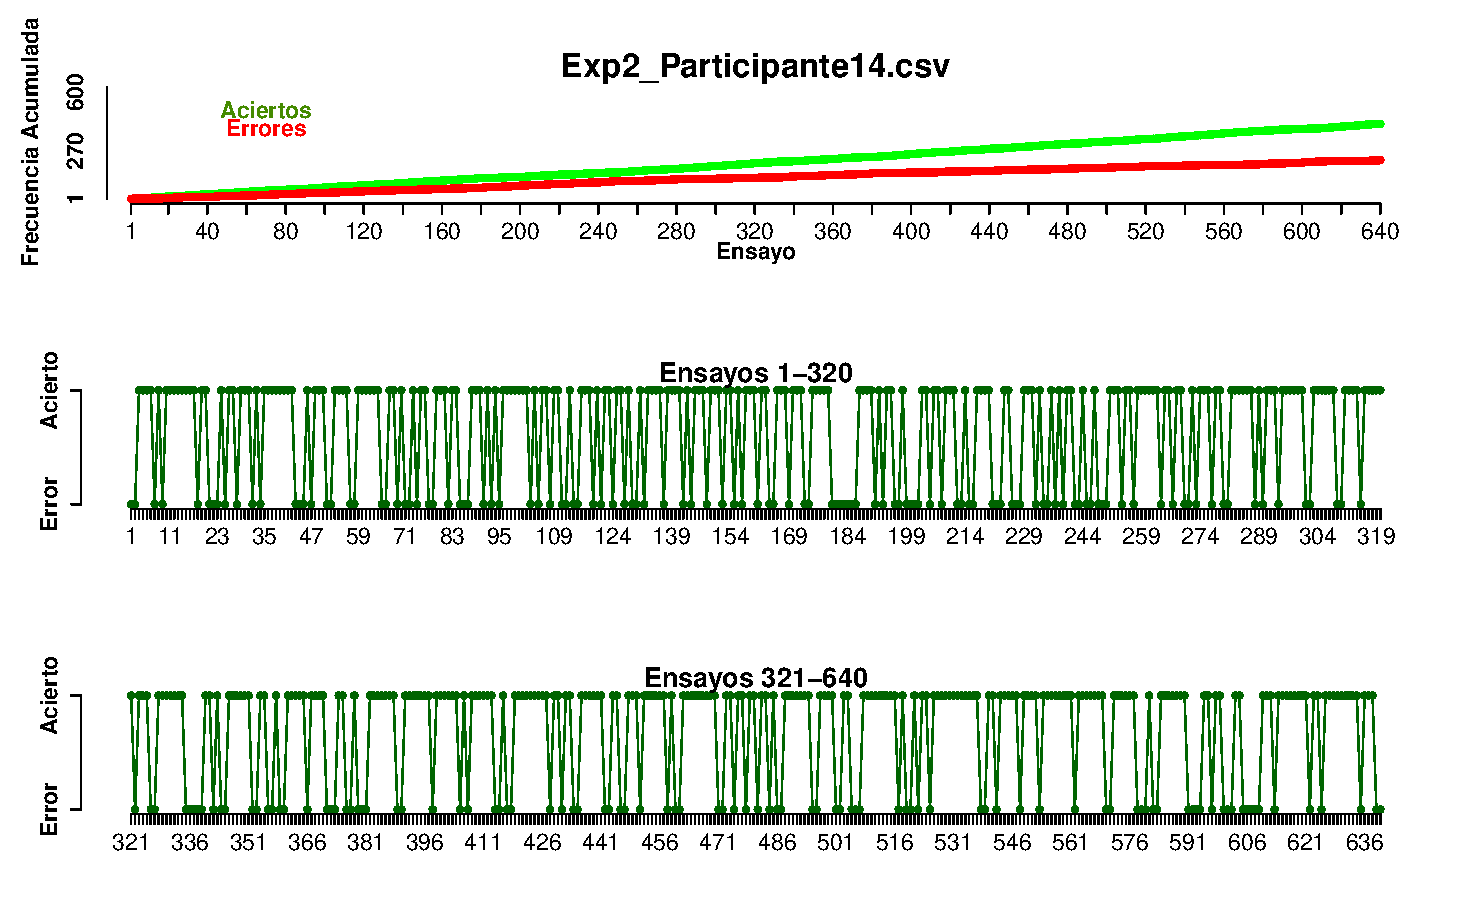
\includegraphics[width=0.60\textwidth]{Figures/Success_Exp2_P14}
%\decoRule
\caption[Aciertos y errores a lo largo del tiempo: Participante ejemplar]{Aciertos y errores cometidos por el Participante 14 del Experimento 1. En el panel superior se muestra el registro acumulativo de estos a lo largo del experimento, en tanto que los paneles inferiores muestran, ensayo a ensayo, la clasificación de las respuestas del participante como Acierto o Error, de acuerdo con el estímulo evaluado. Al respecto de estos últimos se señala que el panel medio muestra la primera mitad del experimento y el panel inferior, el resto.}
\label{fig:Success_E1_P14}
\end{figure}

%Las Figuras~\ref{fig:Success_E1} y \ref{fig:Success_E2} muestran los aciertos y errores cometidos a lo largo de los experimentos por el resto de los participantes en los Experimentos 1 y 2, respectivamente.\\


\item Resultados a lo largo del tiempo

Además de identificar de las respuestas emitidas por los participantes a lo largo de los experimentos como aciertos o errores, se realizó un gráfico que distinguía entre los dos posibles tipos de aciertos y errores en una tarea de detección (hits o rechazos correctos y falsas alarmas u omisiones, respectivamente).\\ 

La Figura~\ref{fig:Outcome_E1_P14} muestra una vez más la ejecución del Participante 14 del Experimento 2, en términos de los resultados obtenidos (i.e. la etiqueta dada a sus respuestas en relación a si fueron, o no, acertadas) a lo largo de la tarea. El panel superior muestra el registro acumulativo de cada uno de los cuatro posibles resultados a lo largo del experimento, en tanto que el panel inferior muestra el resultado obtenido en cada uno de los ensayos.\\ 

\begin{figure}[th]
\centering
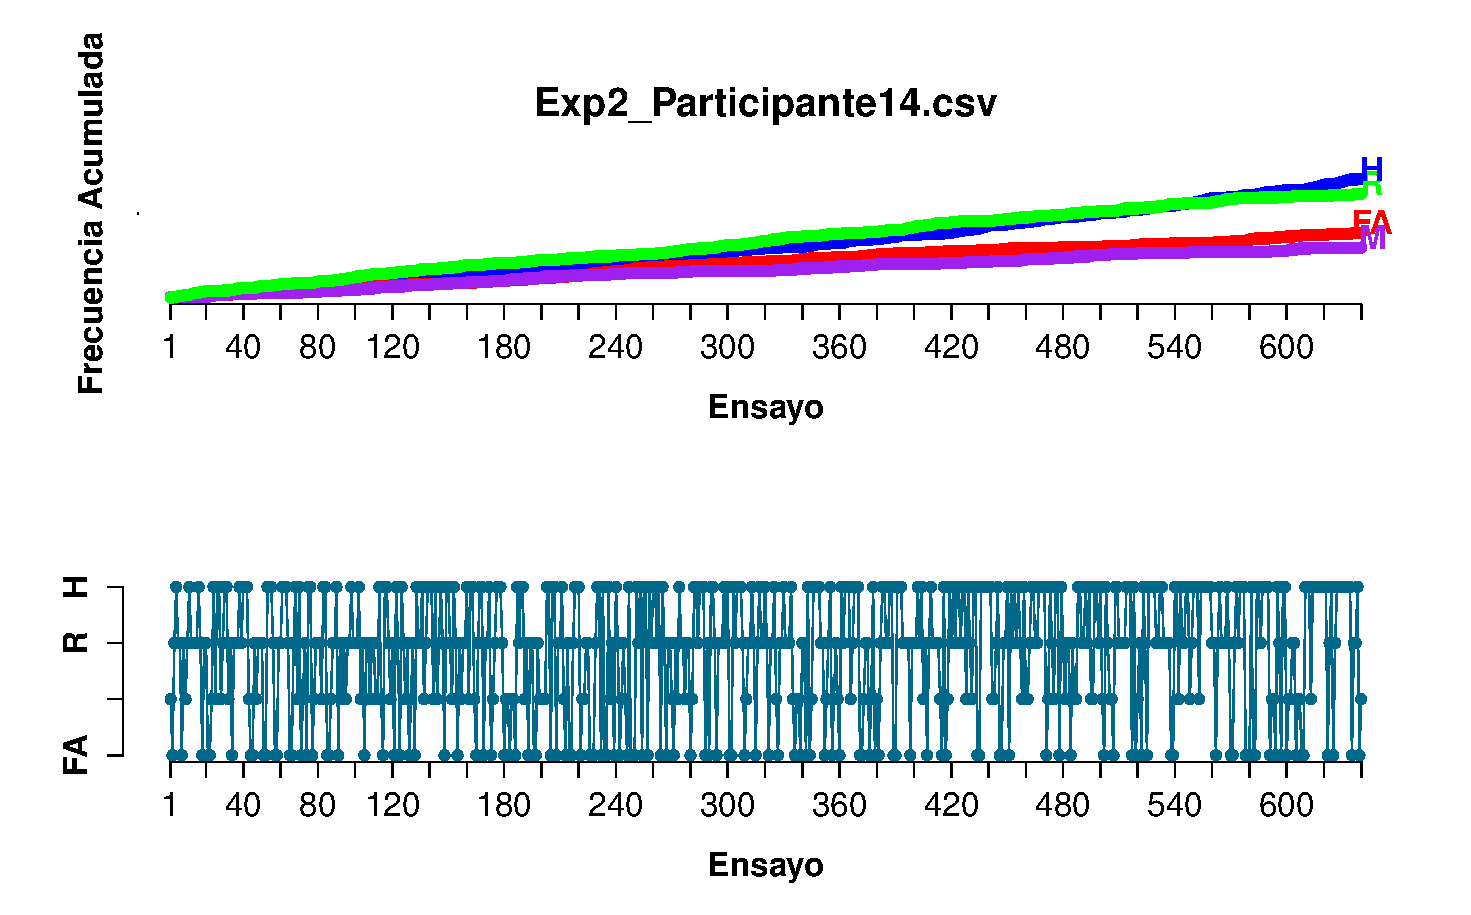
\includegraphics[width=0.60\textwidth]{Figures/Outcome_Exp2_P14}
%\decoRule
\caption[Resultado obtenido a lo largo del tiempo: Ejemplo]{Resultado obtenido por el Participante 6 del Experimento 2, dada cada una de sus respuestas a lo largo del Experimento. El panel superior muestra la frecuencia acumulada de Hits, Falsas Alarmas, Rechazos y Omisiones obtenidos durante el experimento; el panel inferior muestra el tipo de resultado registrado en cada uno de los 640 ensayos.}
\label{fig:Outcome_E1_P14}
\end{figure}

%El resto de los participantes en los experimentos 1 y 2 aparecen en las Figuras~\ref{fig:Outcome_E1} y \ref{fig:Outcome_E2}, respectivamente.\\

\end{itemize}











\subsection{Control 3: ¿Las variables mezcladas para construir los estímulos están afectando el desempeño de los participantes?}

Como se recordará del Capítulo 3, donde se detalla la construcción de los estímulos utilizados en cada uno de los experimentos, la variable deliberadamente manipulada para construir las dos condiciones de dificultad entre las cuales se compara el desempeño de los participantes fue el número de círculos externos en las figuras de Ebbinghaus. Sin embargo, es importante descartar la posibilidad de que el desempeño de los participantes variara en relación a otro tipo de características de los estímulos presentados, como podrían ser los distintos colores en que fueron mostrados cada uno de los estímulos diseñado a lo largo de sus 8 o 10 presentaciones, dependiendo el experimento.\\

\begin{itemize}
\item El efecto del Color sobre la intensidad de la ilusión.

En términos del tipo de influencia que pueden tener las características de los estímulos construidos sobre la ejecución de los participantes, una primer posibilidad es que éstas pudieran estar teniendo un impacto en la intensidad de la ilusión perceptual utilizada. Por ejemplo, sería razonable tener dudas respecto de si los distintos colores en que aparecen cada uno de los estímulos diseñados podría estar alterando la manera en que los participantes responden a los mismos.\\ 

\begin{figure}[th]
\centering
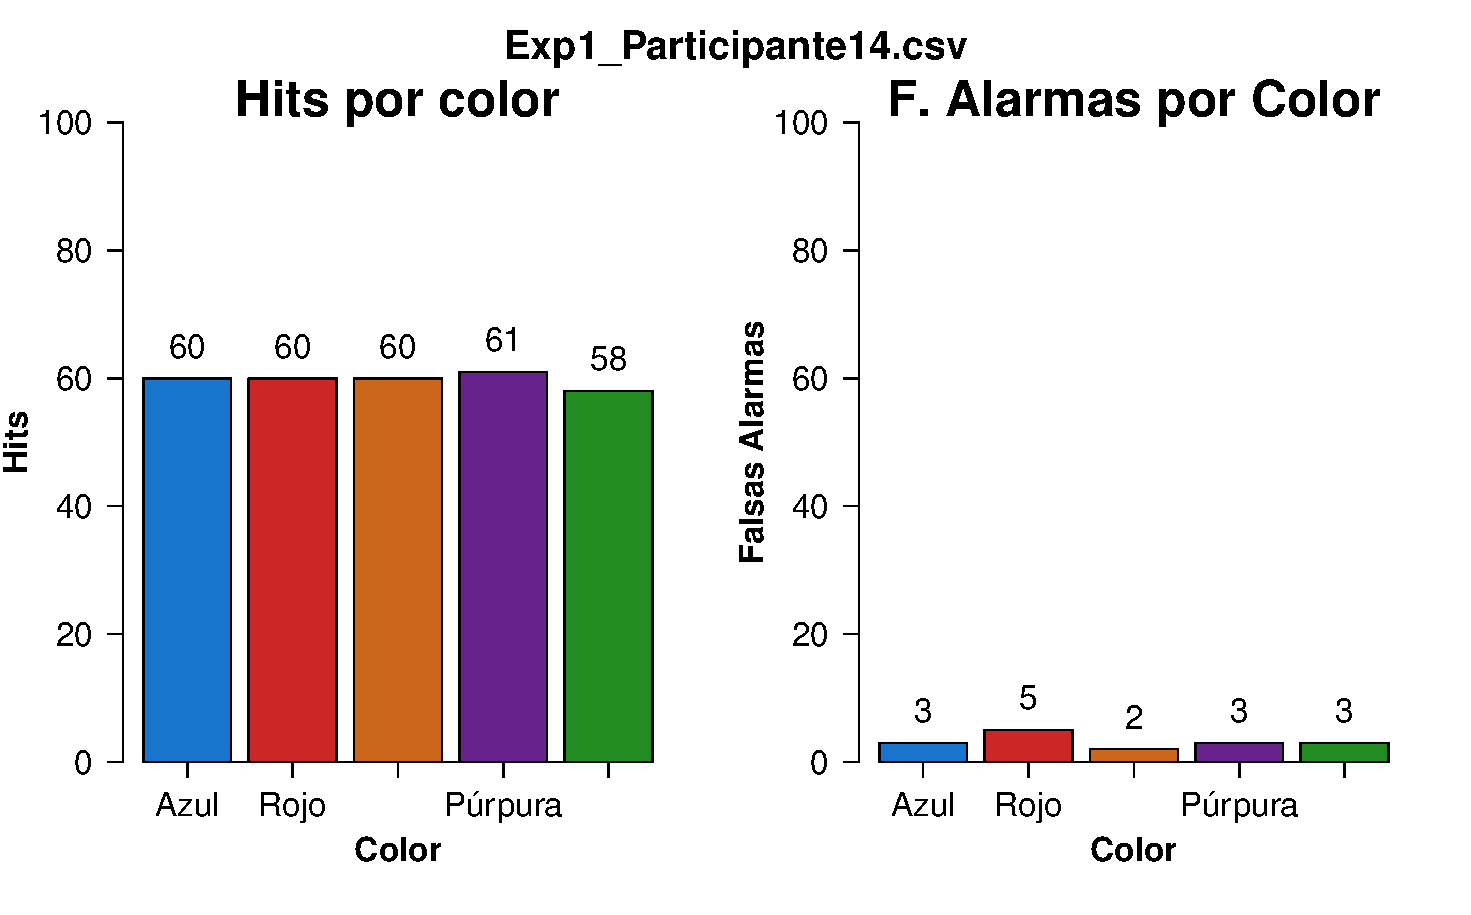
\includegraphics[width=0.60\textwidth]{Figures/Color_Exp1_P14}
%\decoRule
\caption[Hits y Falsas Alarmas por Color; Ejemplo]{Se muestra el desempeño del Participante 14 del Experimento 1 en relación al color de los estímulos. En el panel izquierdo se muestra la relación entre el número de Hits obtenidos y el color de los estímulos, mientras que en el panel derecho se muestra la misma relación para las Falsas alarmas.}
\label{fig:Color_E2_P14}
\end{figure}

La Figura~\ref{fig:Color_E2_P14} muestra la relación entre los Hits y las Falsas alarmas cometidas por el Participante 14 a lo largo del Experimento 2, en relación con el color de las figuras. De acuerdo con las gráficas desplegadas, no parece ser que el color de las figuras tenga un efecto sobre el desempeño de este participante. Se muestran únicamente los Hits y las Falsas Alarmas, pensando que arrojan información suficiente respecto de los aciertos y errores cometidos a lo largo del experimento, en tanto que mantienen una relación complementaria con el número de Omisiones y Rechazos correctos, proporcionando de manera implícita la frecuencia absoluta de estos últimos.\\

%Las gráficas correspondientes a la relación entre las frecuencias absolutas de Hits y Falsas Alarmas y el color de los estímulos, para el resto de los participantes en los Experimentos 1 y 2 se encuentran en la Figura~\ref{fig:Color_E1} y \ref{fig:Color_E2}, respectivamente. 

\item El Efecto del Color sobre la respuesta de los participantes.

Una segunda forma en que el color de los estímulos podría estar alterando el desempeño de los participantes, sería si estos mostraran alguna preferencia a responder de cierta forma ante uno o más de los colores utilizados, con independencia del resto de las características presentes en los estímulos.\\

La Figura~\ref{fig:BiasCol_E1_P13} muestra la proporción de Respuestas 'Sí'/'No' emitidas por el Participante 13 del Experimento 1 para cada uno de los diferentes colores en que fueron presentados los estímulos. Como se puede ver en la figura, parece ser que en general la proporción se mantiene a lo largo de los distintos colores para este participante, por lo que no parece ser que el color esté influyendo en su manera de responder a los estímulos construidos.

\centering
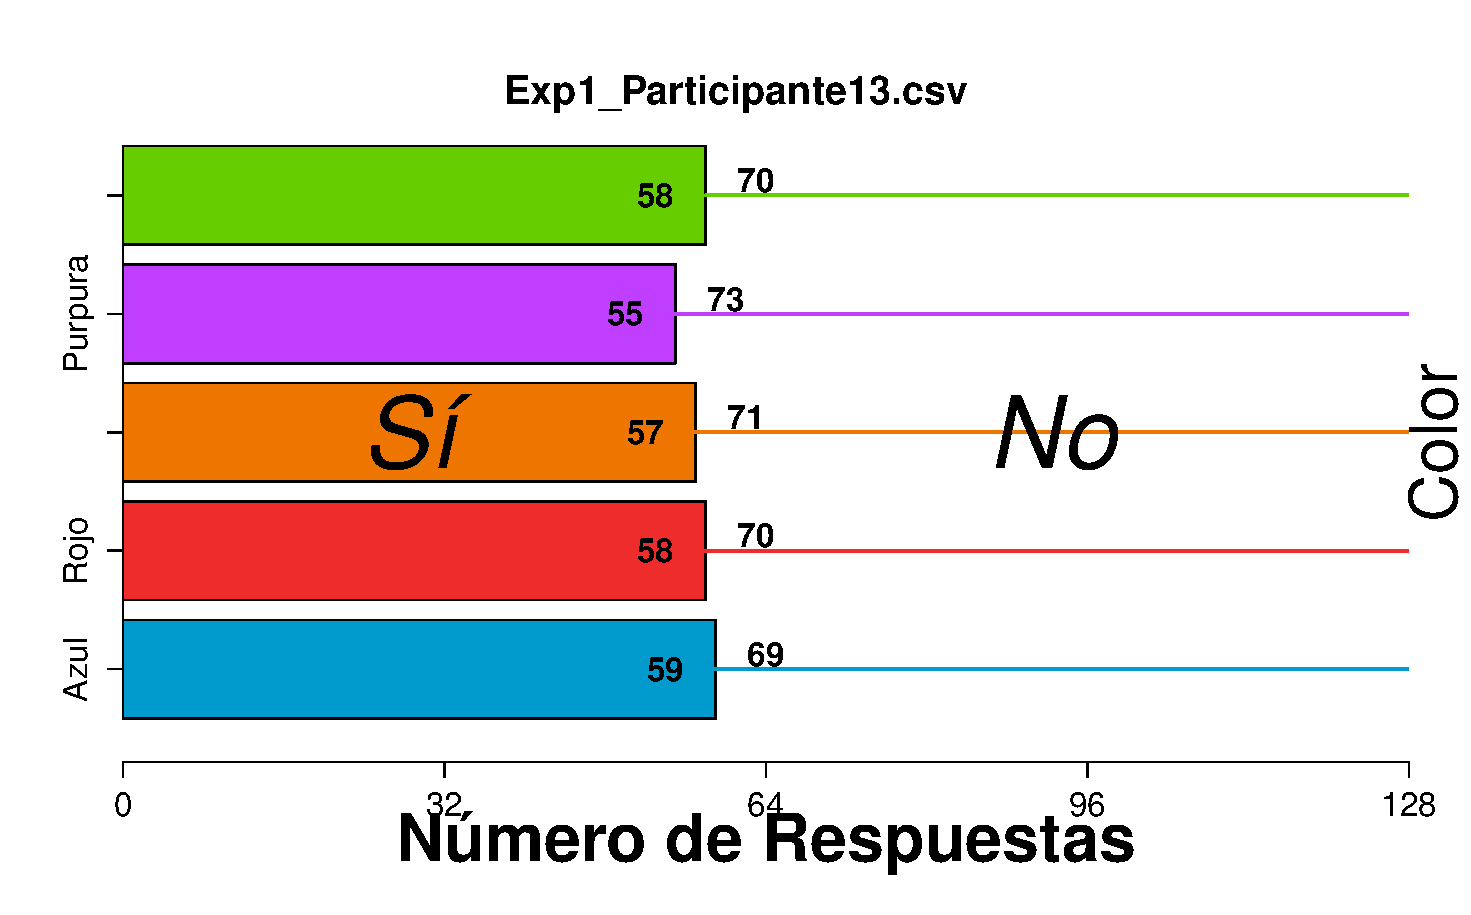
\includegraphics[width=0.40\textwidth]{Figures/BiasColor_Exp1_P13}
%\decoRule
\caption[Proporción de Respuestas 'Sí'/'No' por color; Ejemplo]{Se muestra el desempeño del Participante 14 del Experimento 1 en relación al color de los estímulos. En el panel izquierdo se muestra la relación entre el número de Hits obtenidos y el color de los estímulos, mientras que en el panel dercho se muestra la misma relación para las Falsas alarmas.}
\label{fig:BiasCol_E1_P13}
\end{figure}

%Las Figuras~\ref{fig:BiasCol_E1} y ~\ref{fig:BiasColor_E2} muestran las gráficas correspondientes al resto de los participantes en los Experimentos 1 y 2, respectivamente. 

\end{itemize}


En el Apendice $APENDICE$ se incluyen, a manera de extensión del presente capítulo, todas las gráficas previamente descritas correspondientes al resto de los participantes en los Experimentos 1 y 2.























\section{Análisis estadísticos}


En las tareas contenidas en cada uno de los experimentos realizados (i.e la tarea de detección binaria y la escala de confianza), se encontró evidencia de los patrones de respuesta identificados como parte del Efecto Espejo en al menos tres cuartas partes de los participantes. En el Experimento 1, diecisiete de los veinte participantes mostraron el patrón de respuesta esperado en la tarea de detección binaria y dieciocho en la escala de confianza. A su vez, en el Experimento 2, diecinueve de los veintiun participantes mostraron los patrones asociados con el Efecto Espejo en ambas tareas. De acuerdo a una prueba binomial, todas estas proporciones son estadísticamente significativas contra el azar (p=0.0025 y p=0.0004 para las proporciones reportadas en el Experimento 1, respectivamente; p=0.0002 para el Experimento 2).\\





El análisis de datos está organizado en torno a los siguientes puntos:

\begin{itemize}
\item \textbf{Verificar que las condiciones de dificultad son de hecho diferentes.}
Dado que las condiciones de dificultad fueron diseñadas en función a la literatura revisada en ilusiones ópticas, es preciso corroborar que las manipulaciones implementadas en el diseño de las figuras de Ebbinghaus tuviesen un efecto sobre el desempeño de los participantes. En el marco de la TDS, se esperaría que las discrepancias en la 'dificultad' de la tarea a lo largo de las condiciones construidas, se reflejen en distintos valores del parámetro $d'$ -que cuantifica la discriminabilidad entre señales y ruido como la distancia entre las medias de las distribuciones correspondientes-. En general, se espera encontrar la siguiente relación:
\begin{center}
 D'(A) $>$ D'(B)\\
 \end{center}

 \item \textbf{Comparar las tasas de Hits y Falsas Alarmas entre condiciones.}
Evaluar si, tal y como se reporta en la literatura en memoria de reconocimiento, las diferencias en la ejecución de los participantes entre las dos condiciones de dificultad aparecen 'en dos sentidos', (i.e. en la condición 'fácil' se cometen tanto más aciertos como menos errores, en comparación con la condición con 'difícil'). De acuerdo con la literatura en Memoria de Reconocimiento que aborda el Efecto Espejo, considerando los Hits y las Falsas Alarmas cometidas en cada condición se tomarían como evidencia del mismo los siguientes patrones de respuesta:
\begin{center}
Hits(A) $>$ Hits(B)\\
Falsas Alarmas(B) $>$ Falsas Alarmas(A)\\
\end{center}

\item \textbf{Comparar el puntaje de confianza promedio asignado a cada tipo de ensayo entre las condiciones.}
Además de esperar que las diferencias en el desempeño de los participantes ante dos condiciones de dificultad distintas presentadas de manera ismultánea en la misma tarea se reflejen en los aciertos y errores cometidos en la tarea de detección binaria -de acuerdo con lo reportado en Memoria de Reconocimiento- se espera que estas discrepancias se extiendan a la tarea con la escala de confianza, donde los puntajes asignados por los participantes debieran reflejar sistemáticamente una mayor confianza al responder a los estímulos pertenecientes a la condición fácil que a la condición difícil. Es decir, se espera que:
\begin{center}
Confianza(A) $>$ Confianza(B)\\
\end{center}

Tomando en cuenta que los experimentos fueron programados de manera tal que las respuestas de los participantes respecto a qué tan seguros se sentían sobre la respuesta emitida a la tarea de detección binomial fueran 'traducidas' en puntajes de confianza dentro de una escala más general que distinguía la confianza en sus respuestas negativas ('1', '2' y '3') y la confianza en sus respuestas afirmativas ('4', '5' y '6'), se espera encontrar las siguientes relaciones: \\
\begin{center}
Puntaje(AS) $>$ Puntaje(BS)\\
Puntaje(AN) $<$ Puntaje(BN)\\
\end{center}

\item \textbf{Réplica de controles reportados en la literatura.}
Además de evaluar si las diferencias en la ejecución de los participantes entre las condiciones de dificultad son estadísticamente significativas, en la literatura que reporta evidencia del Efecto Espejo en diversos estudios de memoria de reconocimiento suelen encontrarse controles adicionales añadidos en el análisis de datos como una medida para reafirmar la no-trivialidad del 'efecto reportado' ($REFERENCIA$ ). La importancia de dichos controles se abordará con detalle más adelante. En el presente trabajo de tesis se retoman e incluyen los siguientes:
	\begin{itemize}
	\item Descartar relación entre el tipo de estímulo y los tiempos de respuesta.
	\item Comprobar la extensividad de las diferencias encontradas en la tarea con la escala.
	\end{itemize}
\end{itemize}






Se señala también que el análisis de datos se realizó desde dos enfoques distintos:

\begin{itemize}
\item La réplica de los análisis reportados en la literatura: ANOVA's y Pruebas t\\

Tomando en cuenta que el objetivo princial del trabajo de investigación realizado fue poner a prueba la extensividad de los patrones de respuesta reportados en Memoria de Reconocimiento -identificados como Efecto Espejo- en una tarea de detección perceptual, se consideró pertinente y necesario que los datos obtenidos en los experimentos y tareas planteadas fueran analizados de la misma forma.\\

Se utilizó como guía un artículo publicado por \parencite{Glanzer1990}, donde se reporta evidencia del Efecto Espejo en cinco experimentos en memoria de reconocimiento que difieren en las dimensiones de las palabras cuya manipulación determinó la distinción entre las dos condiciones de dificultad (Palabras poco frecuentes (A) vs Palabras muy frecuentes (B), Significado concreto (A) vs Significado abstracto (B), Interacción con las palabras (A) vs No interacción (B)). Todo el análisis de los datos recabados en la presente investigación fue hecha con una copia de dicho artículo en mano.\\ 

\item El desarrollo de modelos Bayesianos para la estimación paramétrica y la evaluación de la evidencia encontrada.\\



$CITAS LEE$

%Cognitive psychology has a rich set of models for phenomena ranging from low-level vision to high-order problem solving. To a statistician, these cognitive models remain naturally interpretable as statistical models, and in this sense modeling can be considered an elaborate form of data analysis. The dierence is that the models usually are very dierent from default statistical models like general linear models, but instead formalize processes and parameters that have stronger claims to psychological interpretability. There is no clear dividing line between a statistical and a cognitive model. Indeed, it is often possible for the same statistical model to have valid interpretations as a method of data analysis and a psychological model. Signal detection theory is a good example (e.g., Green & Swets, 1966). Originally developed as a method for analyzing binary decisions for noisy signals, in potentially entirely non-psychological contexts, it nonetheless has a natural interpretation as a model of cognitive phenomena like recognition memory. Despite this duality, the distinction between data analysis and psychological modeling is a useful one. The use of Bayesian methods to implement, apply, and evaluate cognitive models is the focus of this chapter.

% Bayesian statistical methods provide a  exible and principled framework  for relating cognitive models to behavioral data. They allow for  cognitive models to be formalized, evaluated, and applied, supporting inferences about parameters, the testing of models, and making  predictions about data. This chapter argues that Bayesian methods are most useful for cognitive modeling in allowing more ambitious accounts of cognition to be considered, including models that include ierarchical, latent-mixture, or common-cause structures. These theoretical possibilities, and the practical mechanics of using Bayesian methods implemented as graphical models, are demonstrated by means of an extended case study, involving psychophysical models of the perception of duration for auditory and visual stimuli. The case study demonstrates a number of general features of the Bayesian approach|representing uncertainty, being sensitive to model complexity, d ealing with contaminants, allowing for individual dierences, making predictions and generalizations, and so on|while emphasizing the role of informative prior distributions to capture theoretical assumptions about cognitive variables, and the complementary roles of parameter inference and model testing in answering research questions

\end{itemize}








\section{Las condiciones de dificultad son diferentes}

Las condiciones de dificultad propuestas para los experimentos realizados, se construyeron con base en los hallazgos reportados por \parencite{Massaro1971} en cuanto al efecto que tienen las diversas variables que componen las figuras de Ebbinghaus. De acuerdo con estos autores, una de las variables cuyo impacto en la intensidad de la ilusión de Ebbinghaus es más claro, es el número de círculos que aparecen en torno al círculo central.

\begin{figure}[th]
\centering
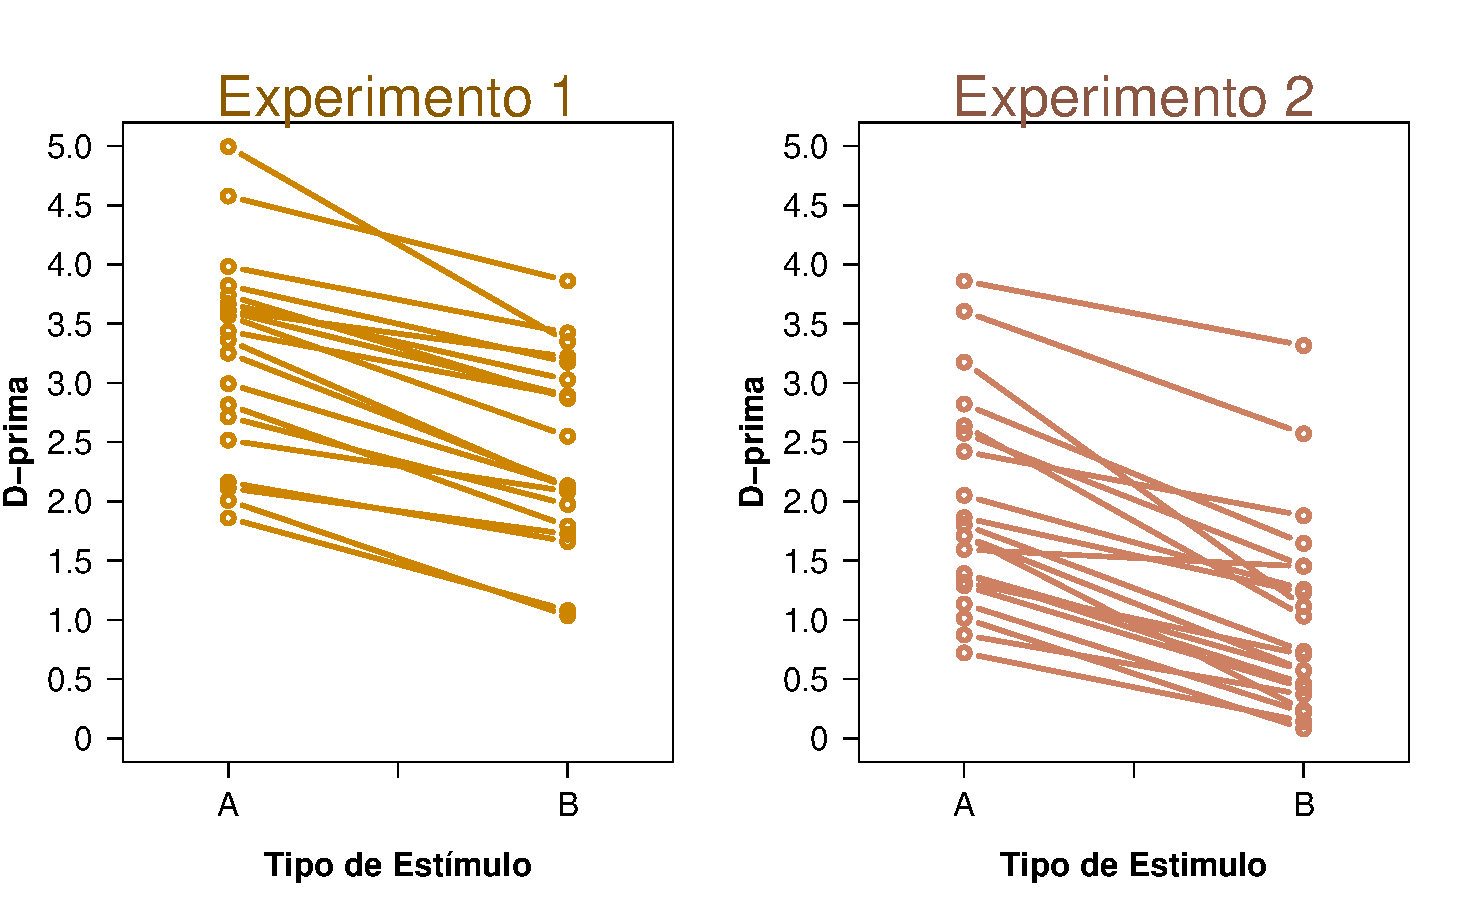
\includegraphics[width=0.80\textwidth]{Figures/Diff_D_E1yE2}
%\decoRule
\caption[Diferencias en Discriminabilidad (Verificando que las condiciones sean, de hecho, diferentes)]{Por cada uno de los experimentos realizados se muestra la relación entre las d' de cada condición de acuerdo a la ejecución de cada uno de los sujetos. En ambos experimentos, se observa una tendencia sistemática a tener mayores niveles de d' en la condición con pocos círculos en las figuras de Ebbinghaus.}
\label{fig:Diff_D}
\end{figure}

\subsection{Análisis 1: Prueba T para comparar las medias de d' por cada condición}

\begin{table}
\caption[Prueba T para evaluar diferencias en las medias de d' entre las condiciones]{Diferencias en d'}
\label{Tabla_t-HitsyFA}
\centering
\begin{tabular}{l | c c c c}
\toprule
%\tabhead{Groups} & \tabhead{Treatment X} & \tabhead{Treatment Y} \\
\textbf{Experimento} & \textbf{$\mu$ A} & \textbf{$\mu$ B} & \textbf{T}  & \textbf{P value}\\
\midrule
Experiment 1 & 3.240 & 2.448 & -3.0587 & 0.0020 \\
Experiment 2 & 1.950 & 1.022 & -3.4972 & 0.0005 \\
\bottomrule
\end{tabular}
\end{table}


\subsection{Análisis 2: Modelo jerárquico bayesiano: Modelo Delta para diferencias en d'}

Se desarrolló un modelo jerárquico bayesiano que asume que las d' y los sesgos C estimados por cada participante en cada una de las condiciones provienen de una distribución normal. El modelo incorpora un parámetro $\delta$ que representa las diferencias entre las medias de las d' estimadas por concidión.

El modelo desarrollado puede verse en la Figura~\ref{fig:Mod_Delta}, estando compuesto por los siguientes elementos:

\begin{itemize}
\item \textbf{Los datos: la materia prima que se señala con nodos sombreados.}
Dado el diseño experimental, conocemos el número total de ensayos con ruido (n) y señal (s). Adicionalmente, por cada participante sabemos cuál es el número total de Hits y Falsas Alarmas cometidos durante el experimento ($H_ij$ y $Fa_ij$, respectivamente). En el modelo, los datos se contienen en nodos cuadrados porque son variables discretas (Nodos circulares indican variables contínuas).\\

\item \textbf{Las tasas como una probabilidad oculta.} 
En la literatura clásica en TDS las tasas de hits y falsas alarmas se interpretan directamente como la proporción de las distribuciones de señal y ruido que caen por encima del criterio ($REFERENCIAS$), respectivamente. Sin embargo, el modelamiento bayesiano nos permite asumir que el número de Hits y Falsas Alarmas observado en cada participante es el resultado de una probabilidad oculta, como parte de un proceso biniomial. Es decir, se asume que el número de Hits y Falsas alarmas

\item \textbf{Sesgo y Discriminabilidad}
De acuerdo con la TDS, las tasas 

\item \textbf{Plato de participantes} 

\item \textbf{Estructura jerárquica:}

\item \textbf{Plato de Condición}

\item \textbf{Parámetro Delta}
\end{itemize} 

\begin{figure}[th]
\centering
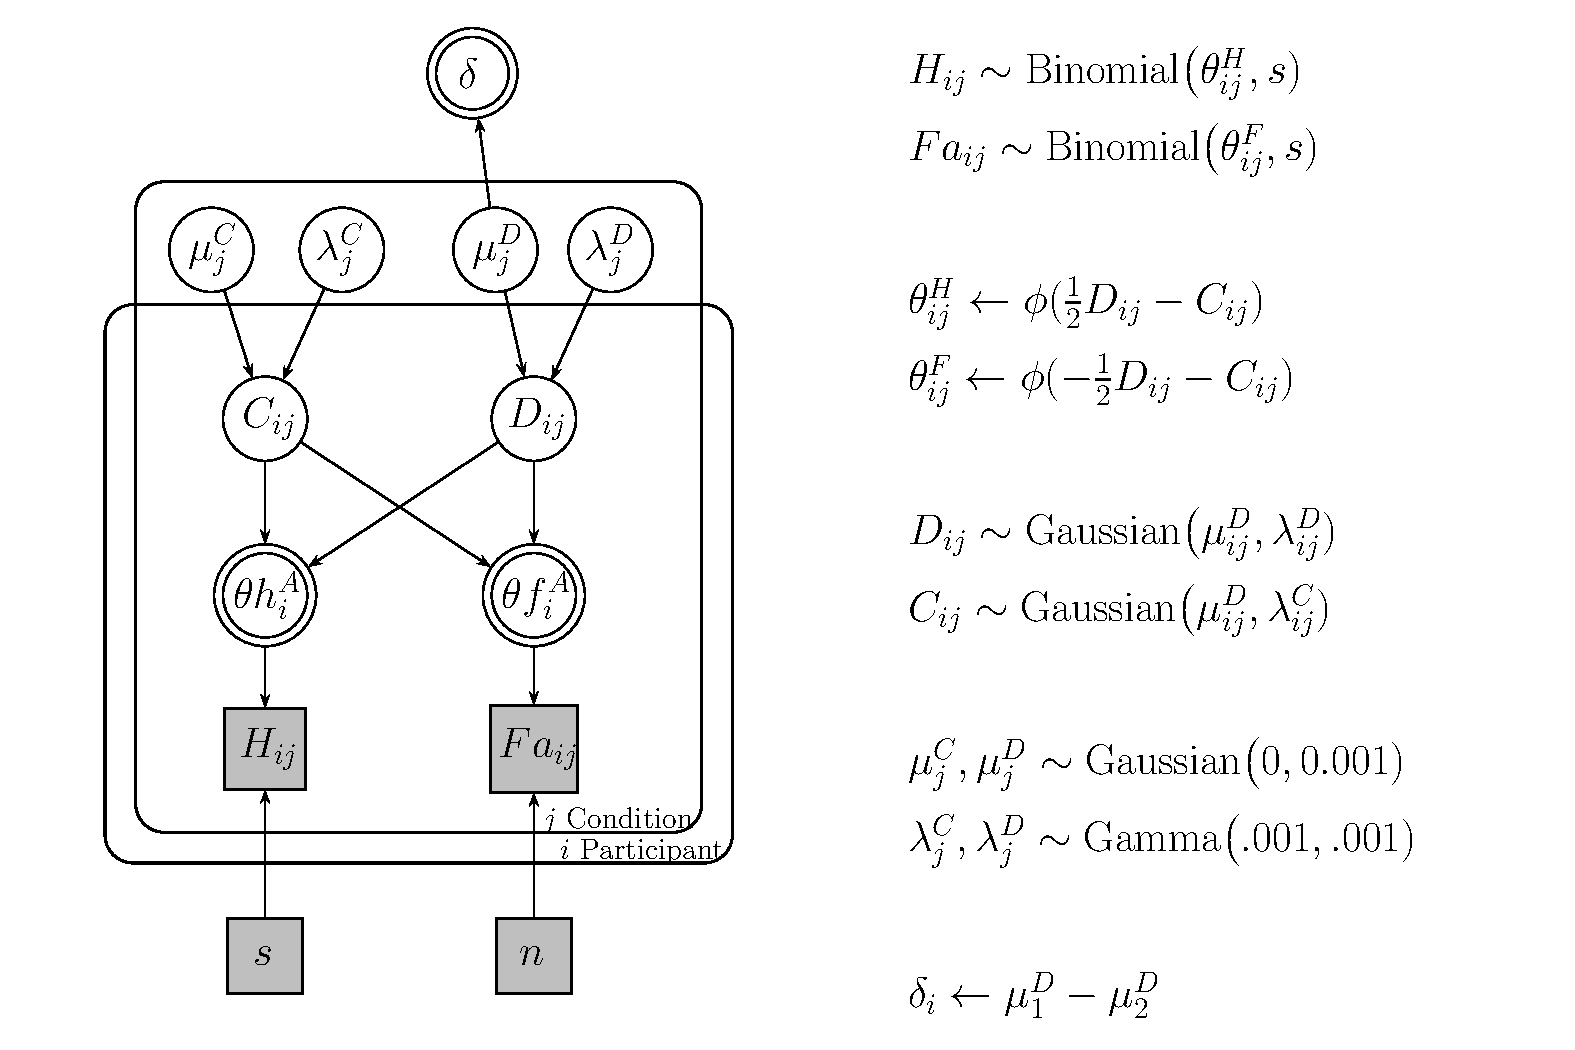
\includegraphics[width=1.1\textwidth]{Figures/Model_Delta_Diff_D}
%\decoRule
\caption[Modelo Delta: Un modelo jerárquico bayesiano para revisar las diferencias en d']{Modelo jerárquico bayesiano con un parámetro Delta ($\delta$) que representa las diferencias en las medias de d' entre las dos condiciones. El modelo tiene priors no informativas.}
\label{fig:Mod_Delta}
\end{figure}









\section{Diferencias en las Tasas de Hits y Falsas Alarmas}




La Figura~\ref{fig:MirrorRate_E2_P4} muestra la frecuencia absoluta de Hits y Falsas Alarmas obtenidas por el Participante 4 en el Experimento 2, en cada una de las condiciones de dificultad puestas a prueba. Como se puede apreciar, este participante muestra claramente el patrón de respuestas identificado como parte del Efecto Espejo en la literatura, siendo que en la condición fácil (A) tiene más aciertos (Hits en AS > Hits en BS) y menos errores (Falsas Alarmas en AN < Falsas Alarmas en BN). Estas discrepancias en el desempeño del participante son consistentes con la idea de que existe una distribución de señal y una distribución de ruido por cada condición de dificultad, que se distribuye en el espacio de elección como un reflejo que se aleja en ambas direcciones, bajo el supuesto de que los participantes están respondiendo a la tarea utilizando un único criterio de elección y que ignoran la existencia de más de un 'tipo de estímulo'.\\

\begin{figure}[th]
\centering
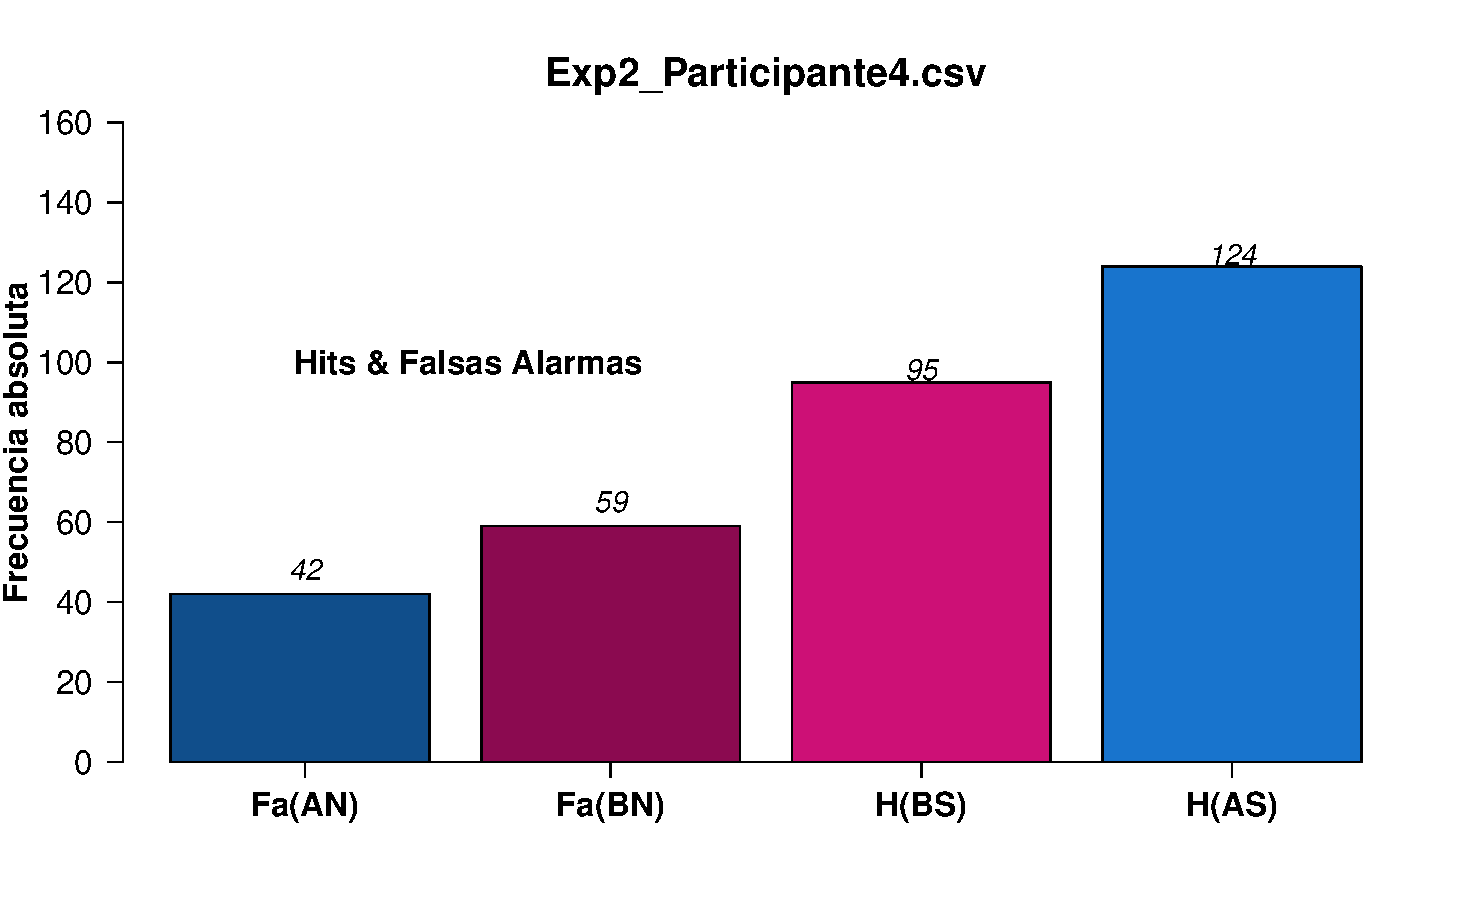
\includegraphics[width=0.60\textwidth]{Figures/MirrorRate_Exp2_P4}
%\decoRule
\caption[Diferencias entre Hits y Falsas Alarmas por Condición; Ejemplo]{Se muestra el desempeño del Participante 14 del Experimento 1 en relación al color de los estímulos. En el panel izquierdo se muestra la relación entre el número de Hits obtenidos y el color de los estímulos, mientras que en el panel derecho se muestra la misma relación para las Falsas alarmas.}
\label{fig:MirrorRate_E2_P4}
\end{figure}




\begin{figure}[th]
\centering
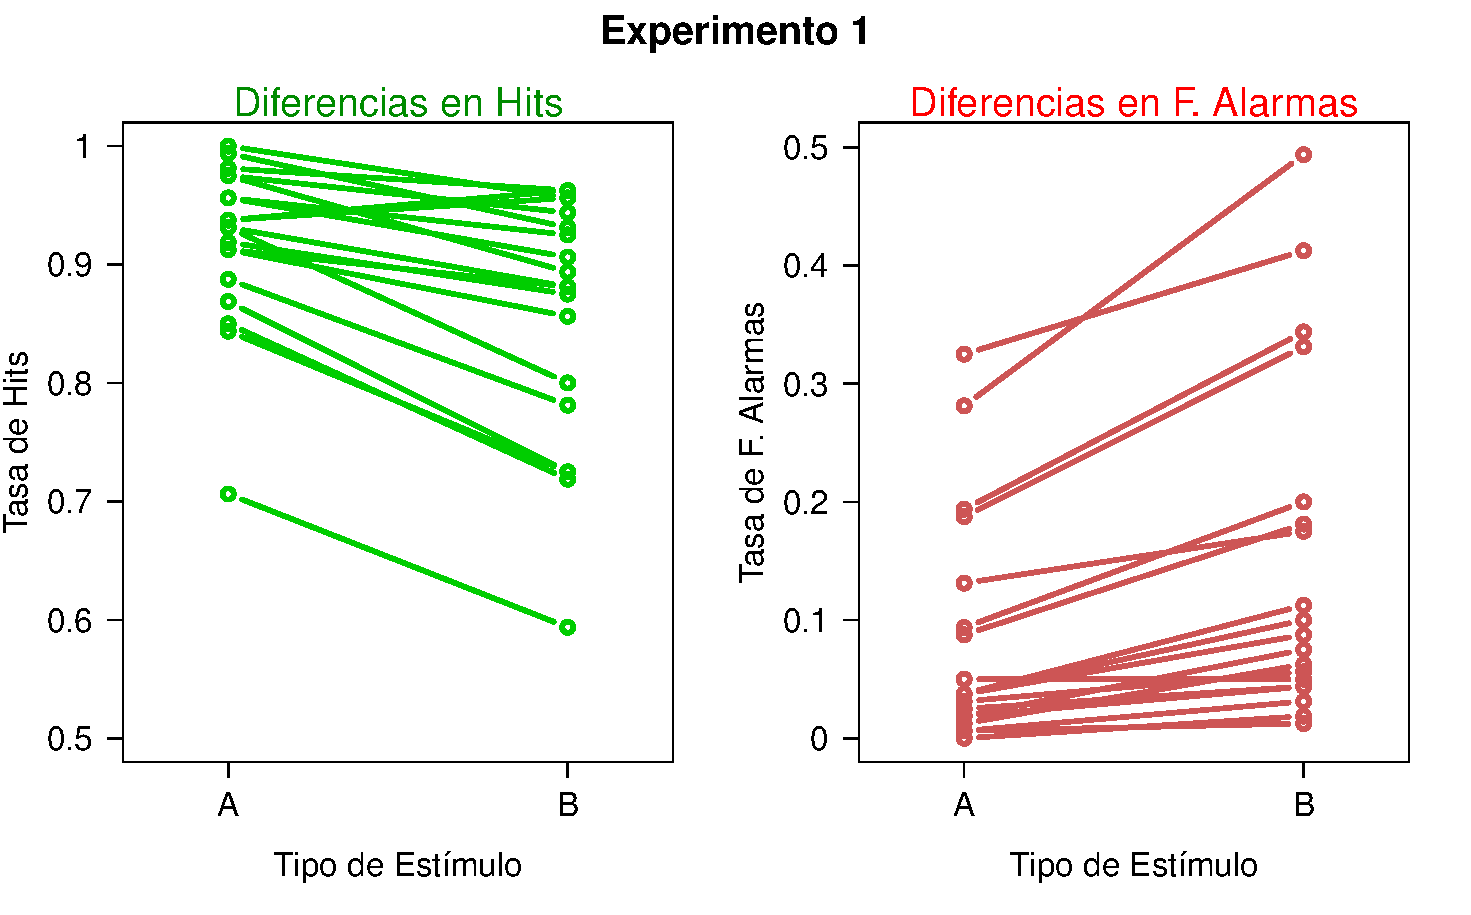
\includegraphics[width=0.80\textwidth]{Figures/Diff_Rate_E1}\\ 
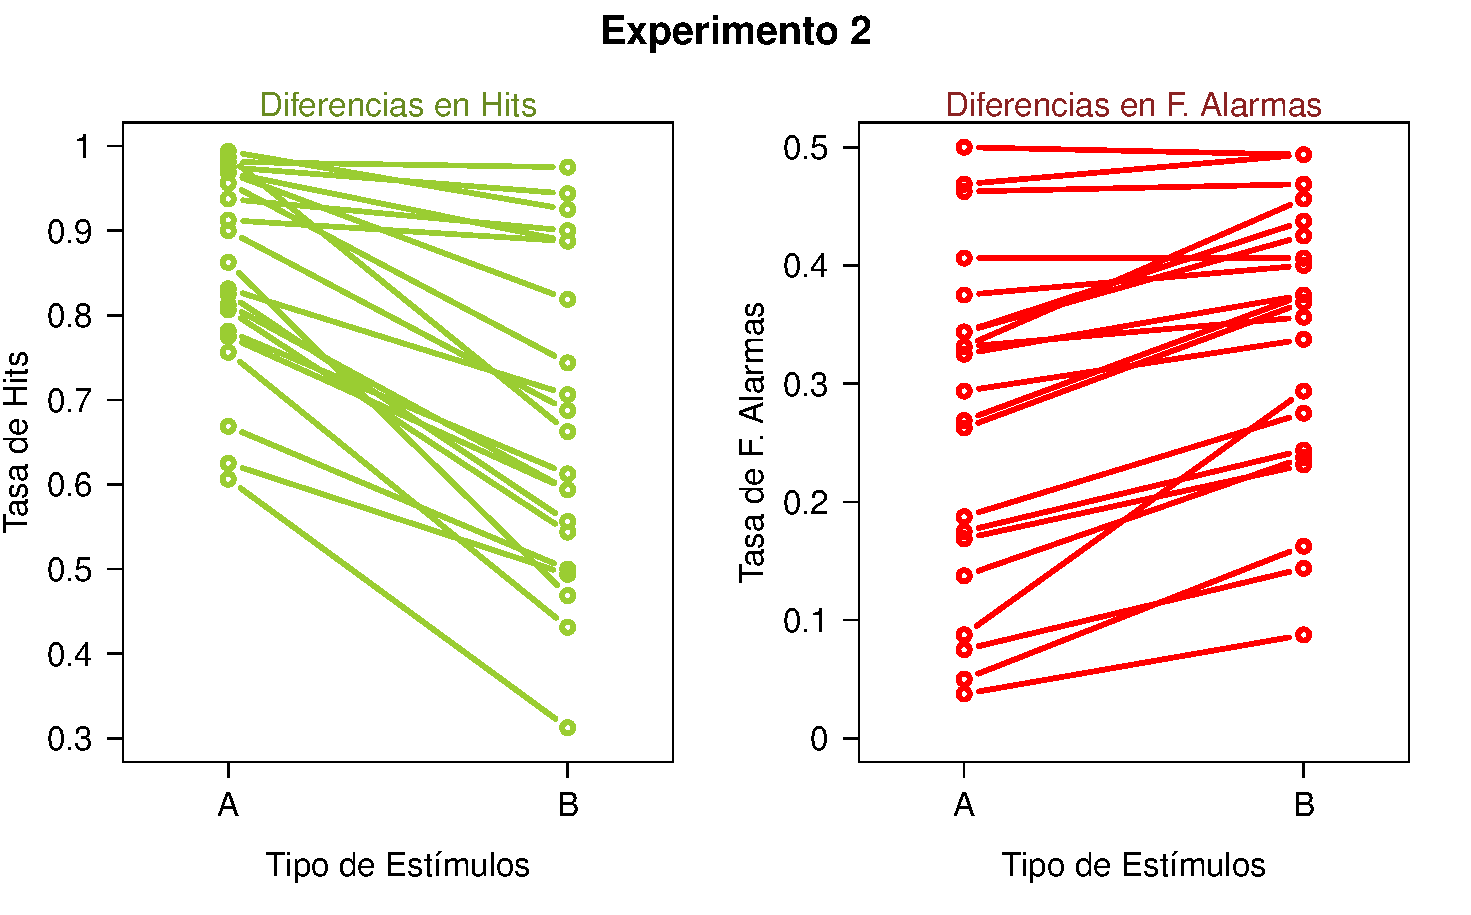
\includegraphics[width=0.80\textwidth]{Figures/Diff_Rate_E2}
%\decoRule
\caption[Diferencias en Tasas (Evaluando diferencias en el desempeño entre las condiciones)]{Comparación intrasujeto de}
\label{fig:Diff_Rate}
\end{figure}


\subsection{Análisis 1: Prueba T}



\begin{table}
\caption[Prueba T para evaluar diferencias en las medias de las tasas de ejecución (Hits y F. Alarmas) entre condiciones]{Diferencias en Hits y Falsas Alarmas entre los tipos de estímulos (Experimento 1 y 2)}
\label{Tabla_t-HitsyFA}
\centering
\begin{tabular}{l l | c c c c}
\toprule
%\tabhead{Groups} & \tabhead{Treatment X} & \tabhead{Treatment Y} \\
\textbf{Experimento} & \textbf{Tasa} & \textbf{$\mu$ A} & \textbf{$\mu$ B} & \textbf{T} & \textbf{P value}\\
\midrule
Exp 1 & Hits & 0.922 & 0.860 & -2.4348 & 0.0098 \\
Exp 1 & FA & 0.08 & 0.143 & 1.917 & 0.0314 \\
Exp 2 & Hits & 0.853 & 0.678 & -3.4757, & 0.0006 \\
Exp 2 & FA & 0.268 & 0.336 & 1.769 & 0.0425 \\
\bottomrule
\end{tabular}
\end{table}


\subsection{Modelo bayesiano}


\begin{figure}[th]
\centering
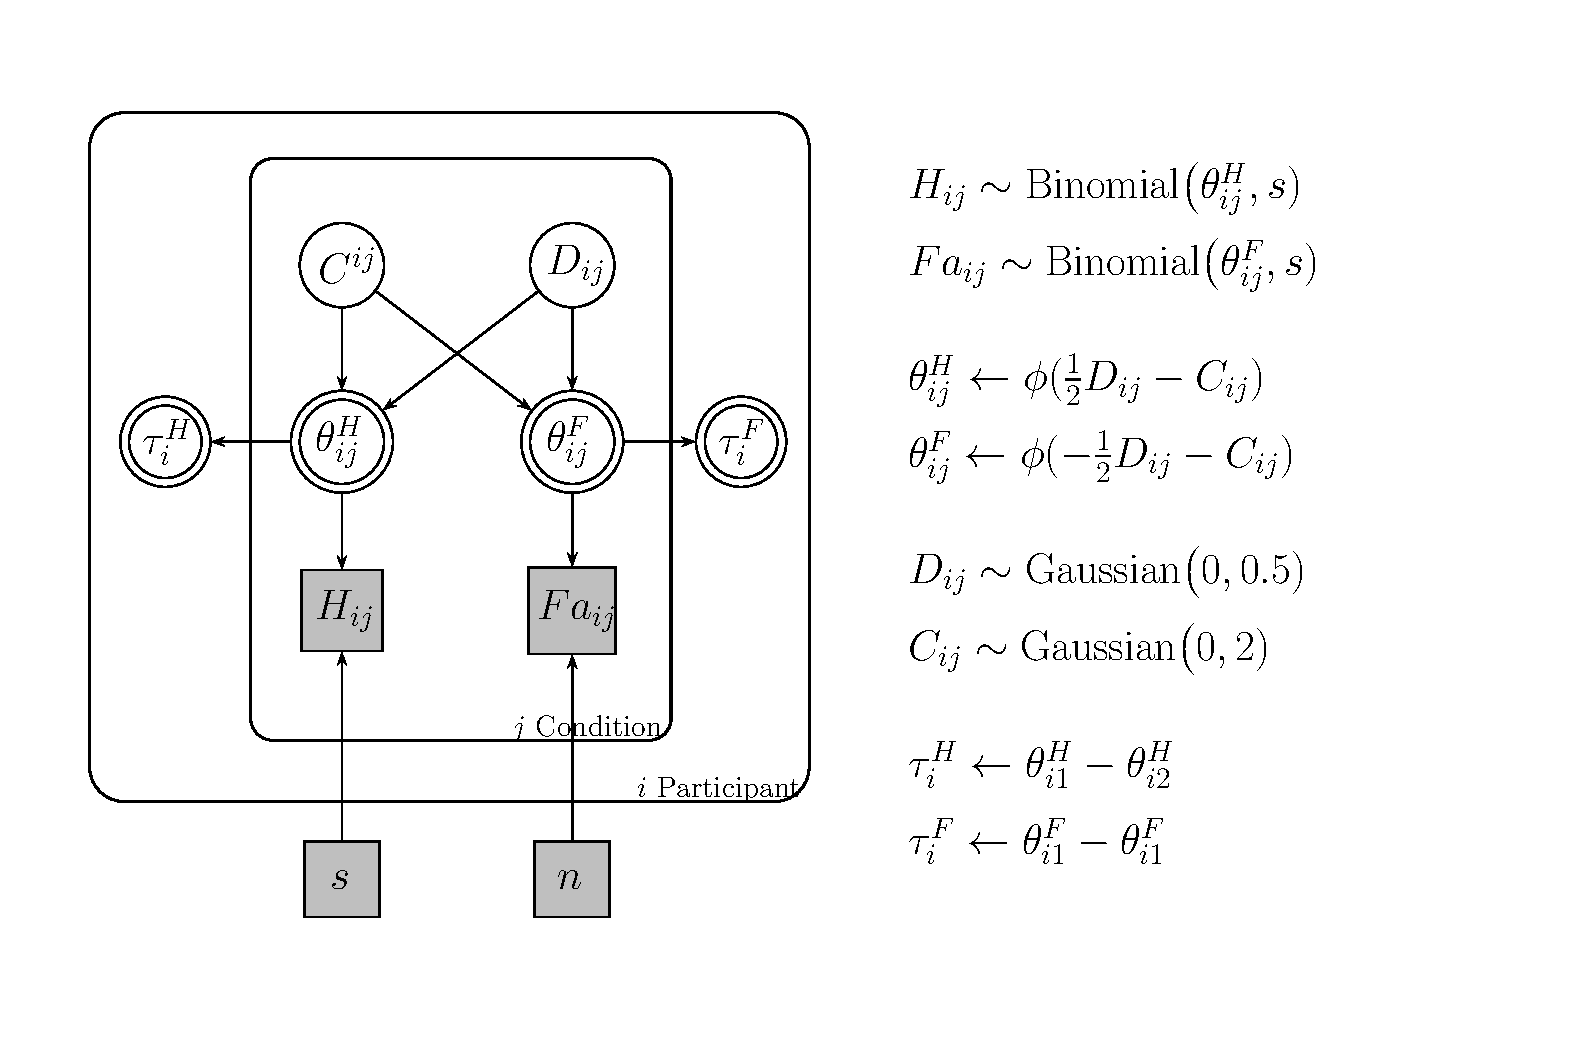
\includegraphics[width=1.1\textwidth]{Figures/Model_Tau_Diff_Tetas}
%\decoRule
\caption[Modelo Tau: Modelo Bayesiano para evaluar las diferencias entre las tasas de hits y falsas alarmas]{Comparación intrasujeto de}
\label{fig:Mod_Tau}
\end{figure}














\section{Diferencias en la asignación de Puntajes de Confianza}


La Figura~\ref{fig:MirrorRating_E1_P10} muestra el promedio de los puntajes de confianza asignados por el Participante 10 del Experimento 1 a los estímulos pertenecientes a cada una de las condiciones de dificultad construidas, separando para cada caso los ensayos con ruido y señal. En la figura puede apreciarse con claridad una tendencia ascendente que coincide con el patrón reportado en estudios de Memoria de Reconocimiento.\\

\begin{figure}[th]
\centering
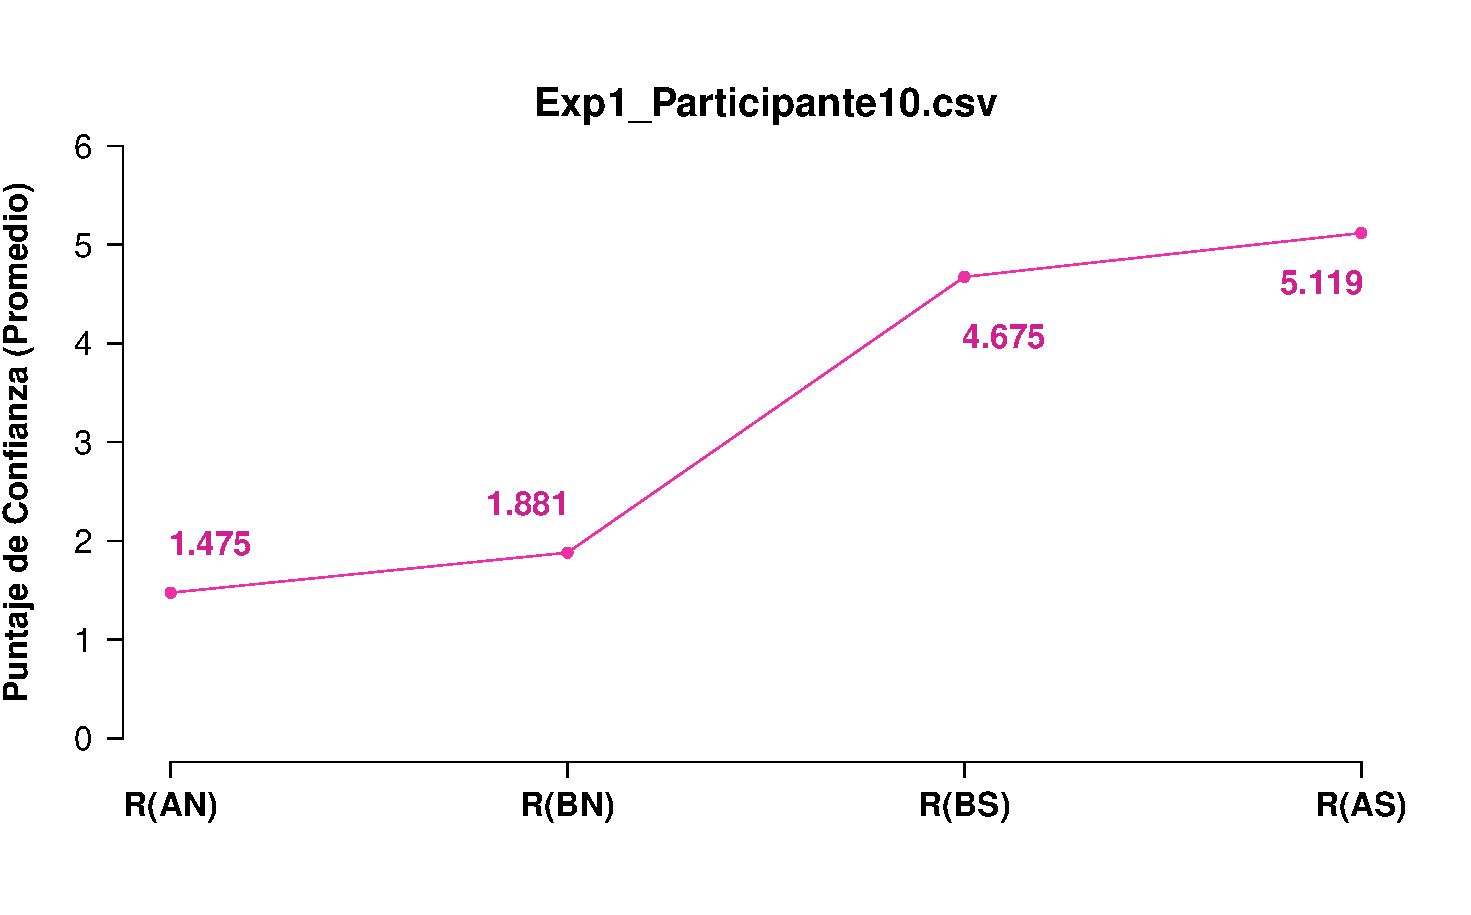
\includegraphics[width=0.60\textwidth]{Figures/MirrorRating_Exp1_P10}
%\decoRule
\caption[Comparación entre Puntajes de Confianza asignados por Condición; Ejemplo]{Se muestra el desempeño del Participante 14 del Experimento 1 en relación al color de los estímulos. En el panel izquierdo se muestra la relación entre el número de Hits obtenidos y el color de los estímulos, mientras que en el panel derecho se muestra la misma relación para las Falsas alarmas.}
\label{fig:MirrorRating_E1_P10}
\end{figure}

%La comparación entre los puntajes de confianza asignados a cada grupo de estímulos por el resto de los participantes en los Experimentos 1 y 2, se presentan en las Figuras~\ref{fig:MERating_E1} y ~\ref{fig:MERating_E2}.\\





\subsection{Análisis 1: }

\begin{table}
\caption[Prueba T para evaluar diferencias en las medias de los puntajes de confianza asigandos entre condiciones]{}
\label{Tabla_t-HitsyFA}
\centering
\begin{tabular}{l l |  c c c c}
\toprule
%\tabhead{Groups} & \tabhead{Treatment X} & \tabhead{Treatment Y} \\
\textbf{Experimento} & \textbf{Ensayo} & \textbf{$\mu$ A} & \textbf{$\mu$ B} & \textbf{T} & \textbf{P value}\\
\midrule
Exp 1 & Signal & 5.445 & 5.212 & -1.7778, & 0.0418 \\
Exp 1 & Noise & 1.542 & 1.883 & -1.7208 & 0.0472 \\
Exp 2 & Signal & 5.183 & 4.342  & -3.6752, & 0.0004 \\
Exp 2 & Noise & 2.386 & 2.752 & -1.809 & 0.0391 \\
\bottomrule
\end{tabular}
\end{table}












\section{Réplica de controles reportados en la literatura}



